\documentclass{journalstyle}




\title{Tests for an Increasing Trend in the Intensity of a Poisson Process: A Power Study}
\author{Maxime Baba, Mathile Ferreira, Félix Foucher de Brandois}
\newcommand{\footertext}{Formation ModIA - INSA, 5$^{\text{th}}$ year \\ 2024-2025}

\begin{document}


\maketitle

%\tableofcontents
%\listoffigures



%\section*{Introduction}

A Nonhomogeneous Poisson Process (NHPP) is a stochastic process often used to model phenomena where the rate of occurrence of events changes over time.
The rate, or intensity function $\lambda(t)$, represents the expected number of events per unit time at a given time $t$.
Understanding and analyzing the behavior of this rate is crucial in diverse fields such as reliability engineering, healthcare, and environmental studies, as it helps identify patterns, predict future events, and optimize interventions \cite{ExampleIntervention}.
Detecting increasing trends in the rate can be particularly important, for example, in monitoring system deterioration or identifying escalating risks in processes.
Although various statistical methods have been proposed to identify increasing trends in NHPPs, existing treatments—such as those by Bain, Engelhardt, and Wright \cite{BainEngelhardtWright}—lack clarity and precision in both theoretical explanation and practical application.
This study addresses these shortcomings by providing a detailed exploration of the Laplace test and Boswell’s likelihood ratio test.
The paper is structured in three parts: a theoretical discussion of the selected tests, numerical simulations comparing their performance, and an application to real-world data.


\section{Theoretical Framework for Trend Detection Tests}

A statistical test evaluates two competing hypotheses: the null hypothesis $H_0$ (representing the status quo) and the alternative hypothesis $H_1$ (indicating a deviation from $H_0$).
Based on the sample data, a test statistic is computed and compared to a critical threshold.
If the test statistic exceeds this threshold, $H_0$ is rejected in favor of $H_1$. \\
In our case, we test whether the intensity function $\lambda(t)$ of a Poisson process is constant ($H_0$) or increasing ($H_1$).

\subsection{Laplace Test}

Let $(N(t))_{t \geq 0}$ be a Poisson process with intensity function $\lambda(t)$.
We observe $N(t)$ in the interval $[0, T^*]$.
Let $0 < T_1 < T_2 < \ldots < T_n < T^*$ be the ordered observation times. \\

\noindent\textbf{Test Statistic} \\
Under $H_0$, the arrival times $T_1, \ldots, T_n$ (conditioned on $N_{T^*} = n$) behave like order statistics from a uniform distribution.
Specifically: \\
$(T_1, \ldots, T_n) | \{N_{T^*} = n\} \overset{(d)}{=} (U_1, \ldots, U_n)$, where $U_1, \ldots, U_n \underset{i.i.d.}{\sim} \mathcal{U}([0, T^*])$. \\
Therefore, $(\frac{T_1}{T^*}, \ldots, \frac{T_n}{T^*}) | \{N_{T^*} = n\} \overset{(d)}{=} (V_1, \ldots, V_n)$, where $V_1, \ldots, V_n \underset{i.i.d.}{\sim} \mathcal{U}([0, 1])$. \\
Define the Laplace test statistic as: 
\begin{equation}
    F = \frac{1}{T^*} \sum_{i=1}^n T_i.
    \label{eq:laplace_test_statistic}
\end{equation}

By the Central Limit Theorem, under $H_0$,  can be standardized as: 
$Z = \frac{F - \mathbb{E}[F]}{\sqrt{\text{Var}(F)}} = \frac{F - \frac{n}{2}}{\sqrt{\frac{n}{12}}} \sim \mathcal{N}(0, 1)$
for large $n$. \\

\noindent\textbf{Decision Rule} \\
If the intensity $\lambda(t)$ is increasing, the arrival times $T_i$ are expected to cluster towards the end of the interval $[0, T^*]$, making $F$ larger.
Therefore, we reject $H_0$ if $F \geq s_{\alpha}$, where $s_{\alpha}$ is the critical threshold determined as: $s_{\alpha} = \frac{n}{2} + z_{1 - \alpha} \sqrt{\frac{n}{12}}$. \\
with $z_{1 - \alpha}$ being the $(1 - \alpha)$-th quantile of the standard normal distribution. \\

\noindent\textbf{Power} \\
The power of the test is the probability of rejecting $H_0$ when $H_1$ is true. \\
$\pi(\lambda) = \mathbb{P}_{H_1}(F \geq s_{\alpha})$.


\subsection{Boswell's Likelihood Ratio Test}

The goal of Boswell's test is to maximize the likelihood function under the constraint that the intensity function $\lambda(t)$ is non-decreasing.
Since the likelihood function involves the intensity values at the observed failure times, we look for the optimal estimates $\hat{\lambda}(T_i)$ that satisfy this constraint. \\

Let $(N(t))_{t \geq 0}$ be a Poisson process with intensity function $\lambda(t)$.
Consider the number $N_{T^*}$ of of "events" that have occurred in $[0, T^*]$, and denote $T_1, \ldots, T_{N_{T^*}} < T^*$ the corresponding arrival times. \\


\noindent\textbf{Likelihood Function Recap} \\
The likelihood function for the observation times $T_1, \ldots, T_n$, conditioned on $N_{T^*} = n$, is given by:
$$
\mathcal{L}((N_t)_{t \in [0, T^*]}; \lambda) = \left(\prod_{i=1}^n \lambda(T_i)\right) \exp\left(-\int_0^{T^*} \lambda(t) dt\right)
$$

We assume that the intensity function $\lambda(t)$ is piecewise constant and non-decreasing between successive failure times $T_{i}$ and $T_{i+1}$.
Therefore, we need to determine the values $\hat{\lambda}(T_i)$ that maximize this likelihood. \\

\noindent\textbf{Formulating the Optimization Problem} \\
Under the previous assumptions (with $T_{n+1} = T^*$): \\
$\int_0^{T^*} \lambda(t) dt = \sum_{i=1}^n (T_{i+1} - T_i) \lambda(T_i)$ \\

\noindent We want to find $\hat{\lambda}(T_i)$ that maximizes: \\
$\prod_{i=1}^{n} \lambda(T_i) \exp(-(T_{i+1} - T_i) \lambda(T_i))$ \\

This can be rewritten as: \\
\begin{equation*}
    \begin{split}
        &\underset{\lambda}{\text{max}} \prod_{i=1}^{n} f_i(\lambda(T_i)) \\
        \text{where } &f_i(x) = x \exp(-(T_{i+1} - T_i) x)
    \end{split}
    \label{eq:boswell_optimization_problem}
\end{equation*}

The function $f_i(x)$ is unimodal, meaning it has a unique maximum.
According to Boswell's theorem \cite{Boswell1966}, following the works of Brunk and von Eeden \cite{VanEeden1956}, the likelihood is maximized by the non-decreasing function $\hat{\lambda}(t)$ given by: \\
\begin{equation*}
    \begin{split}
        &\hat{\lambda}(T_i) = \underset{1 \leq \alpha \leq i}{\text{max}} \underset{i \leq \beta \leq n}{\text{min}} M(\alpha, \beta) \\
        \text{where } &M(\alpha, \beta) \text{ is the maximum of } x \mapsto \prod_{i=\alpha}^{\beta} f_i(x)
    \end{split}
    \label{eq:boswell_optimal_lambda}
\end{equation*}

We can find the form of $M(\alpha, \beta)$ by derviating the product of $f_i(x)$ and setting it to zero. \\
This leads to: \\
\begin{equation}
    \hat{\lambda}(T_i) = \underset{1 \leq \alpha \leq i}{\text{max}} \underset{i \leq \beta \leq n}{\text{min}} \frac{\beta - \alpha + 1}{T_{\beta + 1} - T_{\alpha}}
    \label{eq:boswell_optimal_lambda_formula}
\end{equation}

\noindent\textbf{Test Statistic} \\
The likelihood ratio test (LRT) compares the likelihood of the data under the null hypothesis $H_0$ (constant intensity) with the likelihood under the alternative hypothesis $H_1$ (non-decreasing intensity).
The test statistic is defined as: \\
$$
W = -2 \log \left( \frac{\text{sup }_{\lambda \in \Lambda_0} \mathcal{L}(\lambda)}{\text{sup }_{\lambda \in \Lambda} \mathcal{L}(\lambda)} \right)
$$
where $\Lambda_0$ is the set of constant intensity functions and $\Lambda$ is the set of non-decreasing intensity functions. \\

Under $H_0$, the maximum likelihood estimate of $\lambda(t)$ is $\lambda_0(t) = \frac{N_{T^*}}{T^*} = \frac{n}{T^*}$. \\
The log-likelihood under $H_0$ is:
$$
\log\mathcal{L}(\lambda_0) = \sum_{i=1}^n \log(\lambda_0(T_i)) - T^* \lambda_0 = n \log\left(\frac{n}{T^*}\right) - n
$$

Under $H_1$, the maximum likelihood using the optimal estimate $\hat{\lambda}(t)$ is:
$$
\log\mathcal{L}(\hat{\lambda}) = \sum_{i=1}^n \log(\hat{\lambda}(T_i)) - \int_0^{T^*} \hat{\lambda}(t) dt
$$
By Grenander's lemma \cite{Grenander1956}, we know that: \\
$\int_0^{T^*} \hat{\lambda}(t) dt = n$ \\

Therefore, the test statistic $W$ becomes:
\begin{equation}
    W = 2 \left( \sum_{i=1}^{n} \log(\hat{\lambda}(T_i)) + n \log\left(\frac{T^*}{n}\right) \right)
    \label{eq:boswell_test_statistic}
\end{equation}

According to Wilks' theorem \cite{Wilks1938}, the distribution of the test statistic $W$ asymptotically approaches a $\chi^2$ distribution under the null hypothesis $H_0$.
The degrees of freedom of this distribution are equal to the difference in dimensionality between $\Lambda$ and $\Lambda_0$. \\

We assumed the intensity function $\lambda(t)$ is non-decreasing and can potentially exhibit multiple change points.
Suppose there are $k$ change points, this implies there are $k + 1$ regions where the intensity remains constant.
The possible ways that the $n$ observed failure times can be grouped into $k$ segments are given by the Stirling numbers of the first kind $s(n, k)$ \cite{StirlingNumbers}. \\
We can therefore compute the survival function of the test statistic $W$ under $H_0$ by summing the probabilities of the $\chi^2(k+1)$ distribution for all possible numbers of segments $k$, weighted by the probability of having $k$ segments.
\begin{equation}
    \mathbb{P}_{H_0}(W \geq w) = \sum_{k=1}^{n} \frac{s(n, k)}{n!} \mathbb{P}(\chi^2(k+1) \geq w)
    \label{eq:boswell_survival_function}
\end{equation}


\noindent\textbf{Decision Rule} \\
The decision rule for the LRT is based on the critical threshold $w_{\alpha}$. 
If $W \geq w_{\alpha}$, we reject $H_0$. $w_{\alpha}$ is determined as the $(1 - \alpha)$-th quantile of the previous distribution \eqref{eq:boswell_survival_function}. \\

\noindent\textbf{Power} \\
The power of the test is the probability of rejecting $H_0$ when $H_1$ is true: \\
$\pi(\lambda) = \mathbb{P}_{H_1}(W \geq w_{\alpha})$. \\




\section{Numerical Simulations}

\subsection{Simulation Methodology}

We simulate data from a Nonhomogeneous Poisson Process (NHPP) with various intensity functions $\lambda(t)$:
\begin{itemize}
    \item Exponential trend: $\lambda(t) = e^{\beta t}$, with $\beta \geq 0$
    \item Weibull trend: $\lambda(t) = \beta t^{\beta - 1}$, with $\beta \geq 1$
    \item Step-function trend: $\lambda(t) = \begin{cases}
        1 & \text{if } 0 \leq t \leq \tau \\
        2 & \text{if } \tau < t \leq T^*
    \end{cases}$
\end{itemize}

We generate the arrival times $T_1, \ldots, T_n \in [0, T^*]$ using the inverse transform method.
Then, we perform a Monte Carlo simulation to compare the power of the Laplace test and Boswell's test under different conditions (e.g., sample size, intensity function shape, etc.). \\

\noindent\textbf{Monte Carlo Simulation Principle} \\
\begin{enumerate}
    \item For each scenario (e.g., intensity function, sample size), generate $N$ independent datasets.
    \item For each dataset, apply both the Laplace test and Boswell's likelihood ratio test and record whether the null hypothesis $H_0$ is rejected.
    \item The power $\pi$ of each test is estimated as the proportion of datasets where $H_0$ is rejected: $\pi = \frac{\text{Number of rejections of } H_0}{N}$.
\end{enumerate}




\subsection{Power Analysis}



\subsubsection{Exponential Trend}

The power of the Laplace and Boswell tests is calculated for different values of $\beta$ (). \\
The following figure shows the power curves for the two tests. \\
\begin{figure}[H]
    \centering
    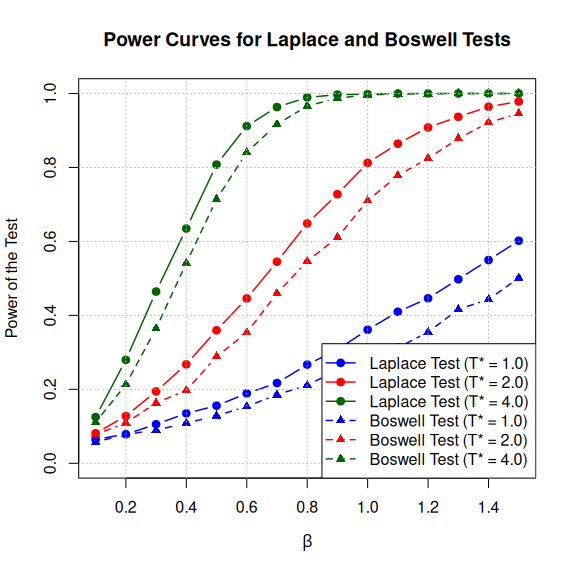
\includegraphics[width=0.3\textwidth]{src/power_exponential.png}
    \caption{Power Curves for Exponential Trend with Different $\beta$}
    \label{fig:power_exponential_beta}
\end{figure}

\textit{ANALYSE}


\subsubsection{Weibull Trend}

The power of the Laplace and Boswell tests is calculated for different values of $\beta$ (). \\
The power curves are plotted to compare the performance of the two tests. \\
\begin{figure}[H]
    \centering
    
\includegraphics[width=0.3\textwidth]{src/power_weibull.png}
    \caption{Power Curves for Weibull Trend with Different $\beta$}
    \label{fig:power_weibull_beta}
\end{figure}

\textit{ANALYSE}


\subsubsection{Step-Function Trend}

The power of the Laplace and Boswell tests is calculated for different values of $\tau$ (). \\
The power curves are plotted to compare the performance of the two tests. \\
\begin{figure}[H]
    \centering
    
\includegraphics[width=0.3\textwidth]{src/power_step_function.png}
    \caption{Power Curves for Step-Function Trend with Different $\tau$}
    \label{fig:power_step_function_tau}
\end{figure}

\textit{ANALYSE}

Discussion of factors influencing the power of each test (sample size, intensity function shape, etc.). \\

Insights into when to prefer one test over the other.





\section{Application to Real-World Data}

\subsection{Description of the Dataset}
Danish Fire Insurance Claims. \\
Overview of the dataset containing large fire insurance claims in Denmark from 1980 to 1990. \\
Explanation of how the event times are extracted and processed.

\subsection{Applying the Tests}
Presentation of test statistics, p-values, and decisions. \\

\subsection{Results and Discussion}
Analysis of Findings. \\
Interpretation of the results and their implications for the intensity of fire insurance claims. \\
Discussion of whether an increasing trend is detected and its significance. \\
Comparison with Simulated Results. \\
Reflecting on how real-world results compare to the numerical simulations.



\section{Conclusion}




\printbibliography


\end{document}